% Define document class
\documentclass[twocolumn]{aastex631}

% Some entries inspired from a preamble by Adrian Price-Whelan, https://github.com/adrn/PhaseSpiralAsteroseismology/blob/main/tex/preamble.tex

\usepackage{showyourwork}

% Latex imports
\let\tablenum\relax             % necessary for AASTeX
\usepackage{siunitx}
\sisetup{range-phrase=-, range-units=single, separate-uncertainty=true}
\sisetup{separate-uncertainty=true}
\usepackage{blindtext}          % Filler text
\usepackage{xcolor}

% paper comments
\usepackage{comment}						 % comments that can be switched visible/invisible
\includecomment{comment}
%\specialcomment{outtake}{\begingroup\sffamily\color{gray}}{\endgroup}
\specialcomment{note}{\begingroup\sffamily\color{red!40!green!70!blue!90}}{\endgroup}
%\excludecomment{note}                       % switch notes off

%% switch TODO notes on/off
\usepackage[backgroundcolor=red!20!green!40!blue!10, textsize=tiny]{todonotes}
\usepackage{regexpatch}
\makeatletter
\xpatchcmd{\@todo}{\setkeys{todonotes}{#1}}{\setkeys{todonotes}{inline,#1}}{}{}
\makeatother
%\usepackage[disable]{todonotes}			% switches all todo notes to invisible

% ---------------------------------
% PAPER VARIABLES
\newcommand{\Nplanets}{\ensuremath{733}}
\newcommand{\percentageTransiting}{999}
\newcommand{\dmax}{\ensuremath{50\,\mathrm{pc}}}
\newcommand{\wrr}{0.001}
\newcommand{\windowsize}{25}
\newcommand{\prSmin}{10}
\newcommand{\prSmax}{1000}
\newcommand{\prWRRmin}{10^{-5}}
\newcommand{\prWRRmax}{0.1}
\newcommand{\prRmin}{0.1}
\newcommand{\prRmax}{15}


% ---------------------------------
% CONSTANTS/MISSIONS/ABBREVIATIONS

% SIunitx definitions
\DeclareSIUnit\mSun{M_\odot}
\DeclareSIUnit\Msun{M_\odot}
\DeclareSIUnit\mStar{M_\star}
\DeclareSIUnit\Mstar{M_\star}
\DeclareSIUnit\mEarth{M_\oplus}
\DeclareSIUnit\Mearth{M_\oplus}
\DeclareSIUnit\rEarth{R_\oplus}
\DeclareSIUnit\Rearth{R_\oplus}
\DeclareSIUnit\year{yr}
\DeclareSIUnit\au{au}
\DeclareSIUnit\dex{dex}
\DeclareSIUnit\ppm{ppm}
\DeclareSIUnit\eV{eV}

% Missions/Projects/Packages
\newcommand{\project}[1]{\textsl{#1}}
\newcommand{\rst}{\project{Nancy Grace Roman Space Telescope}}
\newcommand{\plato}{\project{PLATO}}
\newcommand{\cheops}{\project{CHEOPS}}
\newcommand{\kepler}{\project{Kepler}}
\newcommand{\emcee}{\project{emcee}}

% Stats / probability
\newcommand{\given}{\,|\,}
\newcommand{\norm}{\mathcal{N}}
\newcommand{\pdf}{\textsl{pdf}}

% Maths
\newcommand{\dd}{\mathrm{d}}
\newcommand{\transpose}[1]{{#1}^{\mathsf{T}}}
\newcommand{\inverse}[1]{{#1}^{-1}}
\newcommand{\argmin}{\operatornamewithlimits{argmin}}
\newcommand{\mean}[1]{\left< #1 \right>}

% Non-scalar variables
\renewcommand{\vec}[1]{\ensuremath{\bs{#1}}}
\newcommand{\mat}[1]{\ensuremath{\mathbf{#1}}}

% Unit shortcuts
\newcommand{\msun}{\ensuremath{\mathrm{M}_\odot}}
\newcommand{\mjup}{\ensuremath{\mathrm{M}_{\mathrm{J}}}}
\newcommand{\kms}{\ensuremath{\mathrm{km}~\mathrm{s}^{-1}}}
\newcommand{\mps}{\ensuremath{\mathrm{m}~\mathrm{s}^{-1}}}
\newcommand{\pc}{\ensuremath{\mathrm{pc}}}
\newcommand{\kpc}{\ensuremath{\mathrm{kpc}}}
\newcommand{\kmskpc}{\ensuremath{\mathrm{km}~\mathrm{s}^{-1}~\mathrm{kpc}^{-1}}}
\newcommand{\dayd}{\ensuremath{\mathrm{d}}}
\newcommand{\yr}{\ensuremath{\mathrm{yr}}}
\newcommand{\AU}{\ensuremath{\mathrm{AU}}}
\newcommand{\Kel}{\ensuremath{\mathrm{K}}}

% Misc.
\newcommand{\bs}[1]{\boldsymbol{#1}}

% Astronomy
\newcommand{\feh}{\ensuremath{{[{\rm Fe}/{\rm H}]}}}
\newcommand{\mh}{\ensuremath{{[{\rm M}/{\rm H}]}}}
\newcommand{\logg}{\ensuremath{\log g}}
\newcommand{\Teff}{\ensuremath{T_{\textrm{eff}}}}
\newcommand{\vsini}{\ensuremath{v\,\sin i}}
\newcommand{\gaia}{\textsl{Gaia}}

% Begin!
\begin{document}

% Title
\title{An open source scientific article about extrasolar magma oceans}

% Author list
\author[0000-0001-8355-2107]{Martin Schlecker}
\affiliation{Department of Astronomy/Steward Observatory, The University of Arizona, 933 North Cherry Avenue, Tucson, AZ 85721, USA}
\author{al.}


% Abstract
\begin{abstract}
    $\ldots$ magma oceans $\ldots$

    Here, we assess the ability of space and ground-based telescopes to test this hypothesis using Bioverse, a simulation framework that leverages contextual information from the overall planet population.
    We argue that in the near future, ESA's PLATO mission and NASA's Roman Space Telescope will be the most promising endeavors to constrain this demographic feature.
    For each of these missions, we identify the key mission design drivers that enable a statistically sound detection.
    We also show the unique synergy of these missions in answering this question, and what survey strategy optimizes the statistical power of the combined dataset.

    $\ldots$ its measurement will also provide insights into which stars harbor the nearest habitable worlds.
\end{abstract}

% Main body
\section{Introduction}
\Blindtext[4]

\begin{figure*}
    \begin{centering}
        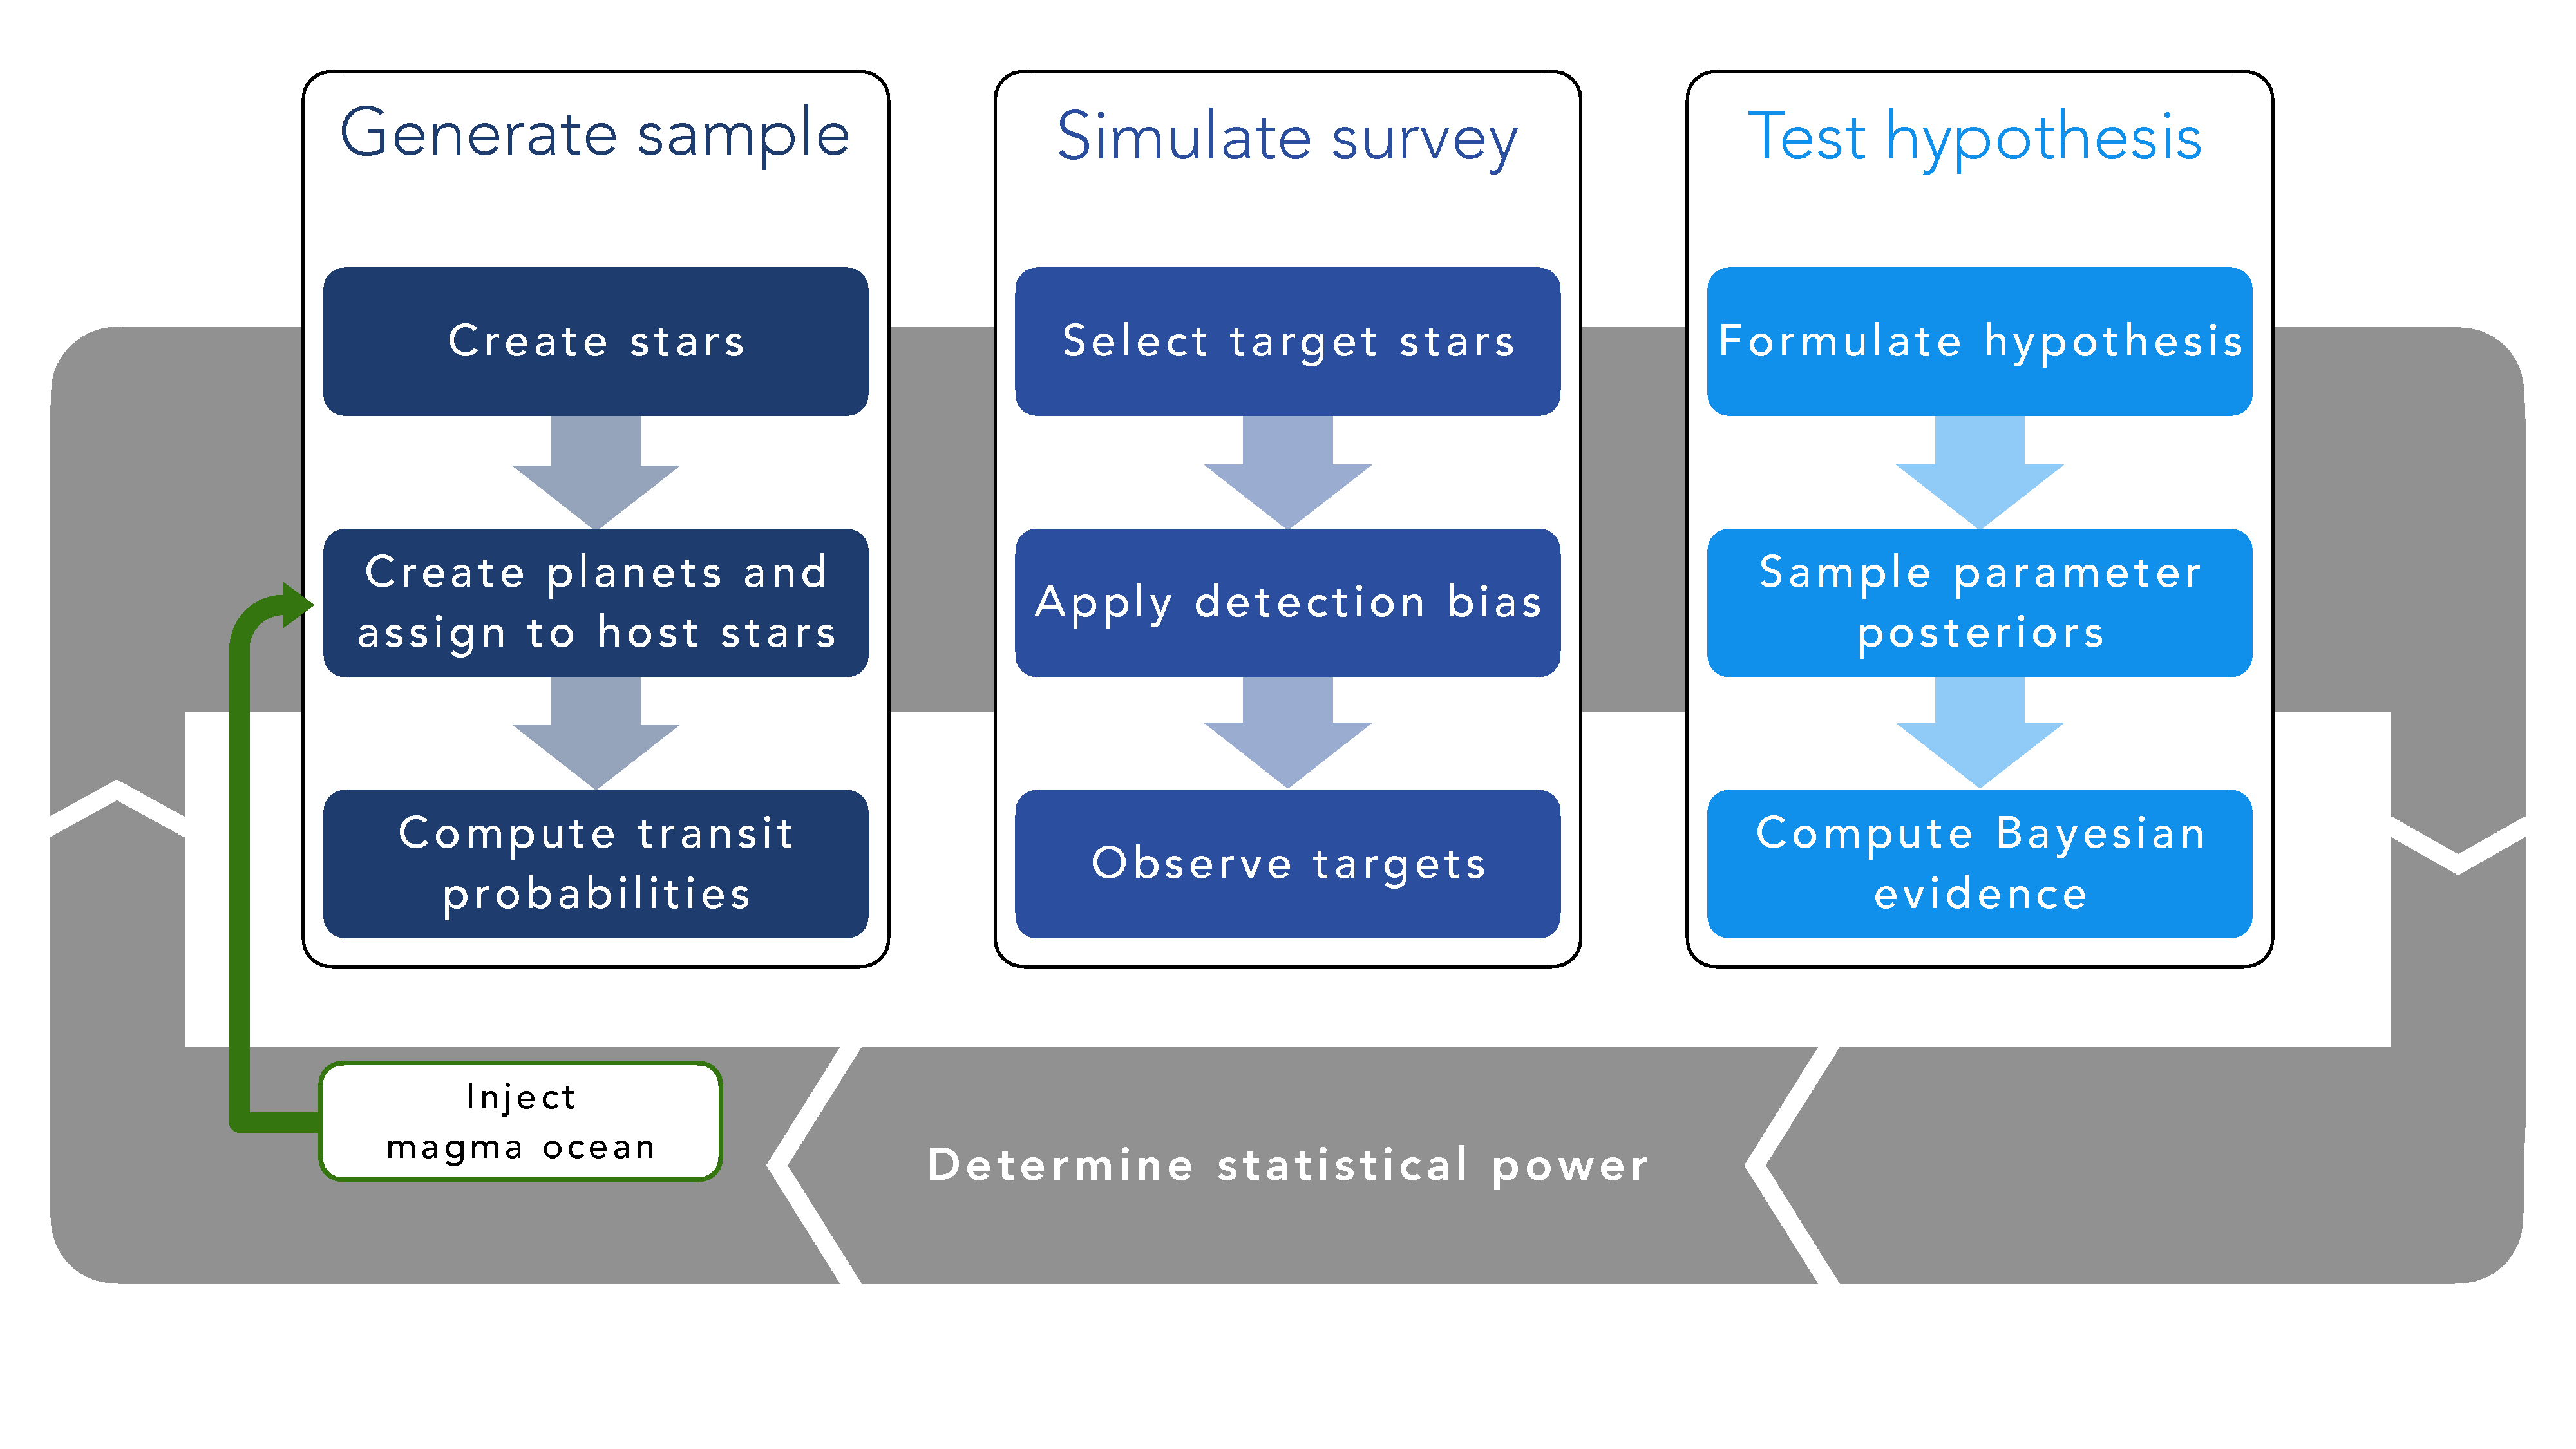
\includegraphics[width=\hsize]{figures/flowchart}
        \caption{Workflow of our hypothesis testing with Bioverse. In the first block, a stellar sample is generated based on XXX. The stars are then populated with planetary systems from XXX, to which a population-level trend can be applied. The planets' respective transit probabilities are computed. The second block simulates the exoplanet survey whereby selection effects and detection biases are introduced. Finally, the third block deals with testing a hypothesis based on the data from the simulated survey. By iterating through these steps, we compute the statistical power of testing the hypothesis given the assumed survey design.}
        \label{fig:flowchart}
    \end{centering}
\end{figure*}

%\begin{deluxetable*}{cc}
%\tablecaption{Confirmed and suggested trends in the exoplanet population}
%%\tablewidth{\pagewidth}
%\tablehead{\colhead{Trend} & \colhead{Reference}}
%\startdata
%missing sub-Saturn mass valley in M-dwarf planetary systems &  Schlecker et al., subm. \\
%$\cdots$ & $\cdots$
%\enddata
%\tablecomments{We show a list of population-level trends that have been reported in demographic studies or predicted from planet formation theories.}
%\end{deluxetable*}
%
%\begin{deluxetable*}{cccccc}
%\tablecaption{Confirmed and suggested trends in the exoplanet population}
%%\tablewidth{\pagewidth}
%\tablehead{\colhead{No.} & \colhead{Trend} & \colhead{Reference} & \colhead{Terrestrials}&\colhead{Roman}&\colhead{Plato}}
%\startdata
%%\hline
%%Theoretically predicted&&&&&
%%\\
%%\hline
%%1&High occurrence of low-mass planets at a few au&\citep{Penny2019}&FALSE&TRUE&FALSE \\
%%2&(super-)Earth occurrence drops again for very low-mass stars&Mulders2021, (Schlecker2021a)&TRUE&TRUE&TRUE
%%\\
%%3&Hot Jupiter - cold Jupiter relation&Schlaufman \& Winn (2016)&FALSE&TRUE&FALSE
%%\\
%%4&super-Earth composition-architecture link&Schlecker+2021a&TRUE&FALSE&FALSE
%%\\
%
%\enddata
%\tablecomments{We show a list of population-level trends that have been reported in demographic studies or predicted from planet formation theories.}
%\end{deluxetable*}



Several patterns in the planetary parameter space have been reported in demographic studies or predicted from planet formation theories.


\section{Synthetic star and planet sample}

\section{The magma ocean hypothesis}

\subsection{Global magma oceans}
\todo[inline]{introduce magma oceans and their influence on planetary radii~\citep{Dorn2021}.\\ Might also be already fully covered in the Introduction section}

\subsection{Demographic imprint of magma oceans}
\todo{describe the expected imprint on the exoplanet population. \\Provide parametrizations from \citet{Dorn2021}'s models.}

\subsubsection{Parametrization}
\todo{specific parametrization, dependency on bulk planet/orbit params (doesn't have to be its own subsubsection)}

\begin{note}
The power from the host star per unit area at the position of a planet or stellar insolation $S$ in units of Earth's insolation is given by
    \begin{equation}
        \frac{S}{S_\oplus} = \left(\frac{L_\star}{L_\odot}\right) \left(\frac{au}{a}\right)^2 .
    \end{equation}

We further define the solar-equivalent semi-major axis $a_{eff} = a (L_\star/L_\odot)^{-1/2}$, at which a planet experiences the same insolation as a Solar System planet at an orbital distance $a$.
\end{note}

\subsection{Synthetic planet populations with and without magma oceans}
\todo{describe the way we inject magma oceans into the synthetic planet population with Bioverse}


\section{Survey simulation}

\subsection{Testing the magma ocean hypothesis with current and planned exoplanet missions}
\todo{PLATO, Ariel, LIFE?, Nautilus\\ What are threshold missions that are able to detect this signal? =>X meter working for Y years, or X' meter working for Y' years => conclusion could be that there is interesting science to do with intermediate size telescope.
 }

\section{Discussion}

\subsection{False positive scenarios}
\todo{what other processes could be confused with a magma ocean signal?}
\begin{note}
Global magma oceans are not the only physical mechanism that may cause a decrease in transit radii for a subset of planets.
Other causes of shrinking planet sizes have been put forward, the most widely discussed ones being atmospheric loss due to either photoevaporation through high-energy radiation by the host star~\citep[e.g.,][]{Owen2013,Jin2014,Mordasini2020a} or due to residual heat from the planet's interior shortly after formation~\citep{Ginzburg2016b,Ginzburg2018,Gupta2019}.
    Both processes are being traded as potentially sculpting the observed radius bimodality of small, close-in exoplanets from the \textit{Kepler} mission~\citep{Fulton2017,VanEylen2018}.
    Like the magma ocean effect discussed here, these processes reduce the radii of some planets, leading to a decrease in average measured planet radii in a specific region of the planetary parameter space.
    This region is distinct from the one affected by global magma oceans, since... \todo{...elaborate why they cannot be confused}

    Another potential false positive contribution comes from the "Neptune desert``, a triangular region of low planet occurrence density of close-in planets in period-radius space~\citep{Szabo2011,Mazeh2016,Dreizler2020b}.
    The shape of this region is such that smaller planets become less frequent the closer to the star they are, which to some degree resembles the pattern introduced by the insolation dependency of the magma ocean probability.
    \todo{explore if this can cause confusion}
\end{note}

\subsection{Mission design trades}\label{sec:mission-design-trades}
\citet{Penny2019} mention that a significant increase in planet yield could be achieved if the telescope's slew speed was increased.

\section{Conclusions}


\bibliographystyle{aasjournal}
\bibliography{bib,PhD}
\end{document}